\documentclass[twoside]{book}

% Packages required by doxygen
\usepackage{fixltx2e}
\usepackage{calc}
\usepackage{doxygen}
\usepackage[export]{adjustbox} % also loads graphicx
\usepackage{graphicx}
\usepackage[utf8]{inputenc}
\usepackage{makeidx}
\usepackage{multicol}
\usepackage{multirow}
\PassOptionsToPackage{warn}{textcomp}
\usepackage{textcomp}
\usepackage[nointegrals]{wasysym}
\usepackage[table]{xcolor}

% Font selection
\usepackage[T1]{fontenc}
\usepackage[scaled=.90]{helvet}
\usepackage{courier}
\usepackage{amssymb}
\usepackage{sectsty}
\renewcommand{\familydefault}{\sfdefault}
\allsectionsfont{%
  \fontseries{bc}\selectfont%
  \color{darkgray}%
}
\renewcommand{\DoxyLabelFont}{%
  \fontseries{bc}\selectfont%
  \color{darkgray}%
}
\newcommand{\+}{\discretionary{\mbox{\scriptsize$\hookleftarrow$}}{}{}}

% Page & text layout
\usepackage{geometry}
\geometry{%
  a4paper,%
  top=2.5cm,%
  bottom=2.5cm,%
  left=2.5cm,%
  right=2.5cm%
}
\tolerance=750
\hfuzz=15pt
\hbadness=750
\setlength{\emergencystretch}{15pt}
\setlength{\parindent}{0cm}
\setlength{\parskip}{0.2cm}
\makeatletter
\renewcommand{\paragraph}{%
  \@startsection{paragraph}{4}{0ex}{-1.0ex}{1.0ex}{%
    \normalfont\normalsize\bfseries\SS@parafont%
  }%
}
\renewcommand{\subparagraph}{%
  \@startsection{subparagraph}{5}{0ex}{-1.0ex}{1.0ex}{%
    \normalfont\normalsize\bfseries\SS@subparafont%
  }%
}
\makeatother

% Headers & footers
\usepackage{fancyhdr}
\pagestyle{fancyplain}
\fancyhead[LE]{\fancyplain{}{\bfseries\thepage}}
\fancyhead[CE]{\fancyplain{}{}}
\fancyhead[RE]{\fancyplain{}{\bfseries\leftmark}}
\fancyhead[LO]{\fancyplain{}{\bfseries\rightmark}}
\fancyhead[CO]{\fancyplain{}{}}
\fancyhead[RO]{\fancyplain{}{\bfseries\thepage}}
\fancyfoot[LE]{\fancyplain{}{}}
\fancyfoot[CE]{\fancyplain{}{}}
\fancyfoot[RE]{\fancyplain{}{\bfseries\scriptsize Generated on Tue Jun 21 2016 17\+:49\+:06 for L\+D\+H by Doxygen }}
\fancyfoot[LO]{\fancyplain{}{\bfseries\scriptsize Generated on Tue Jun 21 2016 17\+:49\+:06 for L\+D\+H by Doxygen }}
\fancyfoot[CO]{\fancyplain{}{}}
\fancyfoot[RO]{\fancyplain{}{}}
\renewcommand{\footrulewidth}{0.4pt}
\renewcommand{\chaptermark}[1]{%
  \markboth{#1}{}%
}
\renewcommand{\sectionmark}[1]{%
  \markright{\thesection\ #1}%
}

% Indices & bibliography
\usepackage{natbib}
\usepackage[titles]{tocloft}
\setcounter{tocdepth}{3}
\setcounter{secnumdepth}{5}
\makeindex

% Hyperlinks (required, but should be loaded last)
\usepackage{ifpdf}
\ifpdf
  \usepackage[pdftex,pagebackref=true]{hyperref}
\else
  \usepackage[ps2pdf,pagebackref=true]{hyperref}
\fi
\hypersetup{%
  colorlinks=true,%
  linkcolor=blue,%
  citecolor=blue,%
  unicode%
}

% Custom commands
\newcommand{\clearemptydoublepage}{%
  \newpage{\pagestyle{empty}\cleardoublepage}%
}


%===== C O N T E N T S =====

\begin{document}

% Titlepage & ToC
\hypersetup{pageanchor=false,
             bookmarks=true,
             bookmarksnumbered=true,
             pdfencoding=unicode
            }
\pagenumbering{roman}
\begin{titlepage}
\vspace*{7cm}
\begin{center}%
{\Large L\+D\+H }\\
\vspace*{1cm}
{\large Generated by Doxygen 1.8.10}\\
\vspace*{0.5cm}
{\small Tue Jun 21 2016 17:49:06}\\
\end{center}
\end{titlepage}
\clearemptydoublepage
\tableofcontents
\clearemptydoublepage
\pagenumbering{arabic}
\hypersetup{pageanchor=true}

%--- Begin generated contents ---
\chapter{Hierarchical Index}
\section{Class Hierarchy}
This inheritance list is sorted roughly, but not completely, alphabetically\+:\begin{DoxyCompactList}
\item \contentsline{section}{App}{\pageref{class_app}}{}
\item \contentsline{section}{Check\+Empty}{\pageref{class_check_empty}}{}
\item \contentsline{section}{File\+Controller}{\pageref{class_file_controller}}{}
\item \contentsline{section}{File\+Controller\+Test}{\pageref{class_file_controller_test}}{}
\item \contentsline{section}{Load\+Files}{\pageref{class_load_files}}{}
\item \contentsline{section}{Tokenizer\+Main}{\pageref{class_tokenizer_main}}{}
\item J\+Frame\begin{DoxyCompactList}
\item \contentsline{section}{Frame}{\pageref{class_frame}}{}
\end{DoxyCompactList}
\item J\+Panel\begin{DoxyCompactList}
\item \contentsline{section}{Panel}{\pageref{class_panel}}{}
\end{DoxyCompactList}
\item Test\+Case\begin{DoxyCompactList}
\item \contentsline{section}{Load\+Files\+Test}{\pageref{class_load_files_test}}{}
\end{DoxyCompactList}
\end{DoxyCompactList}

\chapter{Class Index}
\section{Class List}
Here are the classes, structs, unions and interfaces with brief descriptions\+:\begin{DoxyCompactList}
\item\contentsline{section}{\hyperlink{classapp_1_1_app}{app.\+App} }{\pageref{classapp_1_1_app}}{}
\item\contentsline{section}{\hyperlink{classapp_1_1_check_empty}{app.\+Check\+Empty} }{\pageref{classapp_1_1_check_empty}}{}
\item\contentsline{section}{\hyperlink{classapp_1_1_file_controller}{app.\+File\+Controller} }{\pageref{classapp_1_1_file_controller}}{}
\item\contentsline{section}{\hyperlink{classtests_1_1_file_controller_test}{tests.\+File\+Controller\+Test} }{\pageref{classtests_1_1_file_controller_test}}{}
\item\contentsline{section}{\hyperlink{classapp_1_1_frame}{app.\+Frame} }{\pageref{classapp_1_1_frame}}{}
\item\contentsline{section}{\hyperlink{classapp_1_1_load_files}{app.\+Load\+Files} }{\pageref{classapp_1_1_load_files}}{}
\item\contentsline{section}{\hyperlink{classtests_1_1_load_files_test}{tests.\+Load\+Files\+Test} }{\pageref{classtests_1_1_load_files_test}}{}
\item\contentsline{section}{\hyperlink{classapp_1_1_panel}{app.\+Panel} }{\pageref{classapp_1_1_panel}}{}
\item\contentsline{section}{\hyperlink{classapp_1_1_tokenizer_main}{app.\+Tokenizer\+Main} }{\pageref{classapp_1_1_tokenizer_main}}{}
\end{DoxyCompactList}

\chapter{Class Documentation}
\hypertarget{class_app}{}\section{App Class Reference}
\label{class_app}\index{App@{App}}
\subsection*{Static Public Member Functions}
\begin{DoxyCompactItemize}
\item 
static void \hyperlink{class_app_a941972c4be68395f473d23f1cbf101a7}{main} (String\mbox{[}$\,$\mbox{]} args)
\end{DoxyCompactItemize}


\subsection{Detailed Description}
Clase principal del programa \begin{DoxyAuthor}{Author}
Bianney 
\end{DoxyAuthor}


\subsection{Member Function Documentation}
\hypertarget{class_app_a941972c4be68395f473d23f1cbf101a7}{}\index{App@{App}!main@{main}}
\index{main@{main}!App@{App}}
\subsubsection[{main(\+String[] args)}]{\setlength{\rightskip}{0pt plus 5cm}static void App.\+main (
\begin{DoxyParamCaption}
\item[{String\mbox{[}$\,$\mbox{]}}]{args}
\end{DoxyParamCaption}
)\hspace{0.3cm}{\ttfamily [static]}}\label{class_app_a941972c4be68395f473d23f1cbf101a7}
M�todo principal. Crea una ventana con las distintas opciones que permite ejecutar el programa 
\begin{DoxyParams}{Parameters}
{\em args} & \\
\hline
\end{DoxyParams}


The documentation for this class was generated from the following file\+:\begin{DoxyCompactItemize}
\item 
src/main/java/App.\+java\end{DoxyCompactItemize}

\hypertarget{class_check_empty}{}\section{Check\+Empty Class Reference}
\label{class_check_empty}\index{Check\+Empty@{Check\+Empty}}
\subsection*{Static Public Member Functions}
\begin{DoxyCompactItemize}
\item 
static boolean \hyperlink{class_check_empty_a75322ea66b1c45d81b87f6713a05f655}{check} (J\+Combo\+Box$<$ String $>$ input)
\end{DoxyCompactItemize}


\subsection{Detailed Description}
Clase utilizada para hacer comprobaciones en los J\+Combo\+Box \begin{DoxyAuthor}{Author}
Bianney 
\end{DoxyAuthor}


\subsection{Member Function Documentation}
\hypertarget{class_check_empty_a75322ea66b1c45d81b87f6713a05f655}{}\index{Check\+Empty@{Check\+Empty}!check@{check}}
\index{check@{check}!Check\+Empty@{Check\+Empty}}
\subsubsection[{check(\+J\+Combo\+Box$<$ String $>$ input)}]{\setlength{\rightskip}{0pt plus 5cm}static boolean Check\+Empty.\+check (
\begin{DoxyParamCaption}
\item[{J\+Combo\+Box$<$ String $>$}]{input}
\end{DoxyParamCaption}
)\hspace{0.3cm}{\ttfamily [static]}}\label{class_check_empty_a75322ea66b1c45d81b87f6713a05f655}
M�todo que comprueba si un J\+Combo\+Box tiene seleccionado alg�n elemento 
\begin{DoxyParams}{Parameters}
{\em input} & J\+Combo\+Box a comprobar \\
\hline
\end{DoxyParams}
\begin{DoxyReturn}{Returns}
Booleano que representa si el combo\+Box est� o no vac�o 
\end{DoxyReturn}


The documentation for this class was generated from the following file\+:\begin{DoxyCompactItemize}
\item 
src/main/java/Check\+Empty.\+java\end{DoxyCompactItemize}

\hypertarget{class_file_controller}{}\section{File\+Controller Class Reference}
\label{class_file_controller}\index{File\+Controller@{File\+Controller}}
\subsection*{Public Member Functions}
\begin{DoxyCompactItemize}
\item 
void \hyperlink{class_file_controller_a2a4ed569f4eca8bb41791aa661d1e6a5}{delete\+File} (File file)
\item 
void \hyperlink{class_file_controller_a3167885ae6244993fdbda67468373b25}{add\+Text} (File input)
\item 
void \hyperlink{class_file_controller_a5d06e0c7f8e8852e433c33e0373d6c88}{add} (File output)
\item 
String \hyperlink{class_file_controller_ab4301ad02f998147157e02b465cf5ec3}{file\+To\+String} (File input)
\end{DoxyCompactItemize}
\subsection*{Static Public Attributes}
\begin{DoxyCompactItemize}
\item 
\hypertarget{class_file_controller_aea2e21f282d1c6fc24428305573b4968}{}static String {\bfseries final\+Text} = \char`\"{}\char`\"{}\label{class_file_controller_aea2e21f282d1c6fc24428305573b4968}

\end{DoxyCompactItemize}


\subsection{Detailed Description}
Clase que se encarga de todas las acciones relativas a los ficheros de entrada y salida \begin{DoxyAuthor}{Author}
Bianney 
\end{DoxyAuthor}


\subsection{Member Function Documentation}
\hypertarget{class_file_controller_a5d06e0c7f8e8852e433c33e0373d6c88}{}\index{File\+Controller@{File\+Controller}!add@{add}}
\index{add@{add}!File\+Controller@{File\+Controller}}
\subsubsection[{add(\+File output)}]{\setlength{\rightskip}{0pt plus 5cm}void File\+Controller.\+add (
\begin{DoxyParamCaption}
\item[{File}]{output}
\end{DoxyParamCaption}
)}\label{class_file_controller_a5d06e0c7f8e8852e433c33e0373d6c88}
Funci�n que a�ade al archivo que se le pasa por par�metro el contenido de la variable est�tica final\+Text 
\begin{DoxyParams}{Parameters}
{\em output} & Archivo en el cual se escribir� el contenido de final\+Text \\
\hline
\end{DoxyParams}
\hypertarget{class_file_controller_a3167885ae6244993fdbda67468373b25}{}\index{File\+Controller@{File\+Controller}!add\+Text@{add\+Text}}
\index{add\+Text@{add\+Text}!File\+Controller@{File\+Controller}}
\subsubsection[{add\+Text(\+File input)}]{\setlength{\rightskip}{0pt plus 5cm}void File\+Controller.\+add\+Text (
\begin{DoxyParamCaption}
\item[{File}]{input}
\end{DoxyParamCaption}
)}\label{class_file_controller_a3167885ae6244993fdbda67468373b25}
Funci�n que a�ade el texto de un fichero de entrada a la variable est�tica final\+Text 
\begin{DoxyParams}{Parameters}
{\em input} & Fichero de entrada \\
\hline
\end{DoxyParams}
\hypertarget{class_file_controller_a2a4ed569f4eca8bb41791aa661d1e6a5}{}\index{File\+Controller@{File\+Controller}!delete\+File@{delete\+File}}
\index{delete\+File@{delete\+File}!File\+Controller@{File\+Controller}}
\subsubsection[{delete\+File(\+File file)}]{\setlength{\rightskip}{0pt plus 5cm}void File\+Controller.\+delete\+File (
\begin{DoxyParamCaption}
\item[{File}]{file}
\end{DoxyParamCaption}
)}\label{class_file_controller_a2a4ed569f4eca8bb41791aa661d1e6a5}
Funci�n que borra el contenido del fichero que se le pasa por par�metro 
\begin{DoxyParams}{Parameters}
{\em file} & Fichero al cual se le borra el contenido \\
\hline
\end{DoxyParams}
\hypertarget{class_file_controller_ab4301ad02f998147157e02b465cf5ec3}{}\index{File\+Controller@{File\+Controller}!file\+To\+String@{file\+To\+String}}
\index{file\+To\+String@{file\+To\+String}!File\+Controller@{File\+Controller}}
\subsubsection[{file\+To\+String(\+File input)}]{\setlength{\rightskip}{0pt plus 5cm}String File\+Controller.\+file\+To\+String (
\begin{DoxyParamCaption}
\item[{File}]{input}
\end{DoxyParamCaption}
)}\label{class_file_controller_ab4301ad02f998147157e02b465cf5ec3}
Funci�n que devuelve en un String el contenido de un fichero de texto 
\begin{DoxyParams}{Parameters}
{\em input} & \\
\hline
\end{DoxyParams}
\begin{DoxyReturn}{Returns}

\end{DoxyReturn}


The documentation for this class was generated from the following file\+:\begin{DoxyCompactItemize}
\item 
src/main/java/File\+Controller.\+java\end{DoxyCompactItemize}

\hypertarget{class_file_controller_test}{}\section{File\+Controller\+Test Class Reference}
\label{class_file_controller_test}\index{File\+Controller\+Test@{File\+Controller\+Test}}
\subsection*{Public Member Functions}
\begin{DoxyCompactItemize}
\item 
void \hyperlink{class_file_controller_test_a54702eb8682d933e341ad2dc5f7d8385}{test\+File\+Controller} ()
\end{DoxyCompactItemize}


\subsection{Detailed Description}
Clase que implementa un test para la clase \hyperlink{class_file_controller}{File\+Controller} \begin{DoxyAuthor}{Author}
Bianney 
\end{DoxyAuthor}


\subsection{Member Function Documentation}
\hypertarget{class_file_controller_test_a54702eb8682d933e341ad2dc5f7d8385}{}\index{File\+Controller\+Test@{File\+Controller\+Test}!test\+File\+Controller@{test\+File\+Controller}}
\index{test\+File\+Controller@{test\+File\+Controller}!File\+Controller\+Test@{File\+Controller\+Test}}
\subsubsection[{test\+File\+Controller()}]{\setlength{\rightskip}{0pt plus 5cm}void File\+Controller\+Test.\+test\+File\+Controller (
\begin{DoxyParamCaption}
{}
\end{DoxyParamCaption}
)}\label{class_file_controller_test_a54702eb8682d933e341ad2dc5f7d8385}
Test que comprueba que la función file\+To\+String(\+File) devuelve el valor esperado. 

The documentation for this class was generated from the following file\+:\begin{DoxyCompactItemize}
\item 
src/test/java/File\+Controller\+Test.\+java\end{DoxyCompactItemize}

\hypertarget{class_frame}{}\section{Frame Class Reference}
\label{class_frame}\index{Frame@{Frame}}
Inheritance diagram for Frame\+:\begin{figure}[H]
\begin{center}
\leavevmode
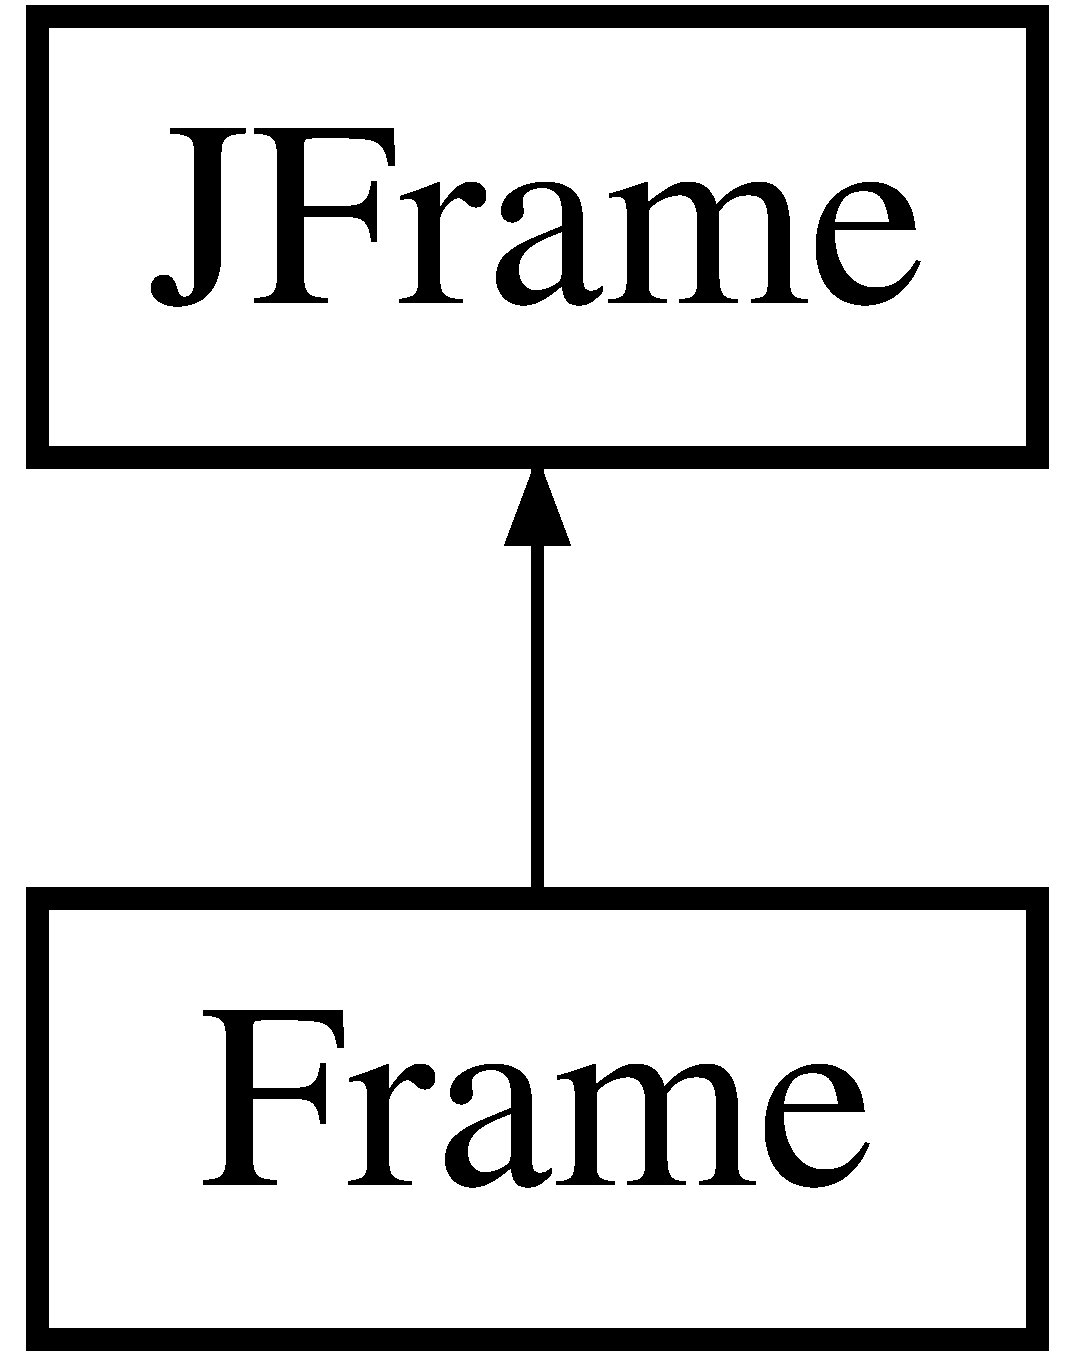
\includegraphics[height=2.000000cm]{class_frame}
\end{center}
\end{figure}
\subsection*{Public Member Functions}
\begin{DoxyCompactItemize}
\item 
\hyperlink{class_frame_a271be43afe808c2eed83766472da276a}{Frame} (J\+Panel panel, String title)
\end{DoxyCompactItemize}


\subsection{Detailed Description}
Clase que contiene la ventana de la interfaz gr�fica del programa \begin{DoxyAuthor}{Author}
Bianney 
\end{DoxyAuthor}


\subsection{Constructor \& Destructor Documentation}
\hypertarget{class_frame_a271be43afe808c2eed83766472da276a}{}\index{Frame@{Frame}!Frame@{Frame}}
\index{Frame@{Frame}!Frame@{Frame}}
\subsubsection[{Frame(\+J\+Panel panel, String title)}]{\setlength{\rightskip}{0pt plus 5cm}Frame.\+Frame (
\begin{DoxyParamCaption}
\item[{J\+Panel}]{panel, }
\item[{String}]{title}
\end{DoxyParamCaption}
)}\label{class_frame_a271be43afe808c2eed83766472da276a}
Constructor de la clase. Establece las caracter�sticas de la ventana. 
\begin{DoxyParams}{Parameters}
{\em panel} & \hyperlink{class_panel}{Panel} que recoge el contenido de la ventana \\
\hline
{\em title} & T�tulo que se mostrar� en la ventana \\
\hline
\end{DoxyParams}


The documentation for this class was generated from the following file\+:\begin{DoxyCompactItemize}
\item 
src/main/java/Frame.\+java\end{DoxyCompactItemize}

\hypertarget{class_load_files}{}\section{Load\+Files Class Reference}
\label{class_load_files}\index{Load\+Files@{Load\+Files}}
\subsection*{Static Public Member Functions}
\begin{DoxyCompactItemize}
\item 
static String\mbox{[}$\,$\mbox{]} \hyperlink{class_load_files_adf968969e5533d946b751b8b99008fe1}{load} ()
\end{DoxyCompactItemize}


\subsection{Detailed Description}
Clase que carga los nombres de los ficheros .txt existentes en el directorio input\+Files/ \begin{DoxyAuthor}{Author}
Bianney 
\end{DoxyAuthor}


\subsection{Member Function Documentation}
\hypertarget{class_load_files_adf968969e5533d946b751b8b99008fe1}{}\index{Load\+Files@{Load\+Files}!load@{load}}
\index{load@{load}!Load\+Files@{Load\+Files}}
\subsubsection[{load()}]{\setlength{\rightskip}{0pt plus 5cm}static String \mbox{[}$\,$\mbox{]} Load\+Files.\+load (
\begin{DoxyParamCaption}
{}
\end{DoxyParamCaption}
)\hspace{0.3cm}{\ttfamily [static]}}\label{class_load_files_adf968969e5533d946b751b8b99008fe1}
Funci�n que devuelve un array con los nombres de los ficheros contenidos en el directorio input\+Files \begin{DoxyReturn}{Returns}
Array con los nombres de los ficheros .txt 
\end{DoxyReturn}


The documentation for this class was generated from the following file\+:\begin{DoxyCompactItemize}
\item 
src/main/java/Load\+Files.\+java\end{DoxyCompactItemize}

\hypertarget{class_load_files_test}{}\section{Load\+Files\+Test Class Reference}
\label{class_load_files_test}\index{Load\+Files\+Test@{Load\+Files\+Test}}
Inheritance diagram for Load\+Files\+Test\+:\begin{figure}[H]
\begin{center}
\leavevmode
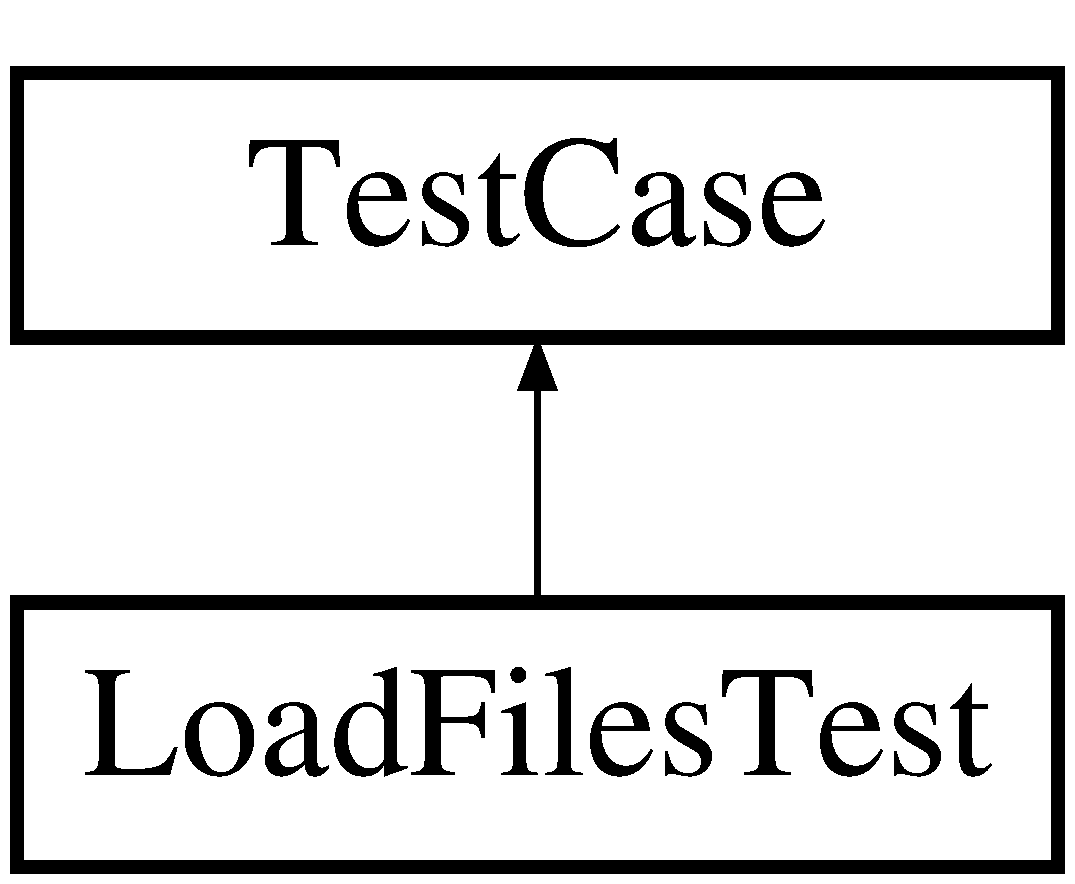
\includegraphics[height=2.000000cm]{class_load_files_test}
\end{center}
\end{figure}
\subsection*{Public Member Functions}
\begin{DoxyCompactItemize}
\item 
void \hyperlink{class_load_files_test_a6041de4a7d56d21845f6ab2318acf9b9}{test\+Load\+Files} ()
\item 
void \hyperlink{class_load_files_test_a735b5ac28080a30e79a747489287c8fc}{test\+Create\+Object} ()
\end{DoxyCompactItemize}


\subsection{Detailed Description}
Clase que implementa tests para la clase \hyperlink{class_load_files}{Load\+Files} \begin{DoxyAuthor}{Author}
Bianney 
\end{DoxyAuthor}


\subsection{Member Function Documentation}
\hypertarget{class_load_files_test_a735b5ac28080a30e79a747489287c8fc}{}\index{Load\+Files\+Test@{Load\+Files\+Test}!test\+Create\+Object@{test\+Create\+Object}}
\index{test\+Create\+Object@{test\+Create\+Object}!Load\+Files\+Test@{Load\+Files\+Test}}
\subsubsection[{test\+Create\+Object()}]{\setlength{\rightskip}{0pt plus 5cm}void Load\+Files\+Test.\+test\+Create\+Object (
\begin{DoxyParamCaption}
{}
\end{DoxyParamCaption}
)}\label{class_load_files_test_a735b5ac28080a30e79a747489287c8fc}
Test que comprueba que un objeto de la clase \hyperlink{class_load_files}{Load\+Files} se ha creado correctamente \hypertarget{class_load_files_test_a6041de4a7d56d21845f6ab2318acf9b9}{}\index{Load\+Files\+Test@{Load\+Files\+Test}!test\+Load\+Files@{test\+Load\+Files}}
\index{test\+Load\+Files@{test\+Load\+Files}!Load\+Files\+Test@{Load\+Files\+Test}}
\subsubsection[{test\+Load\+Files()}]{\setlength{\rightskip}{0pt plus 5cm}void Load\+Files\+Test.\+test\+Load\+Files (
\begin{DoxyParamCaption}
{}
\end{DoxyParamCaption}
)}\label{class_load_files_test_a6041de4a7d56d21845f6ab2318acf9b9}
Test que comprueba el buen funcionamiento de la función load() 

The documentation for this class was generated from the following file\+:\begin{DoxyCompactItemize}
\item 
src/test/java/Load\+Files\+Test.\+java\end{DoxyCompactItemize}

\hypertarget{class_panel}{}\section{Panel Class Reference}
\label{class_panel}\index{Panel@{Panel}}
Inheritance diagram for Panel\+:\begin{figure}[H]
\begin{center}
\leavevmode
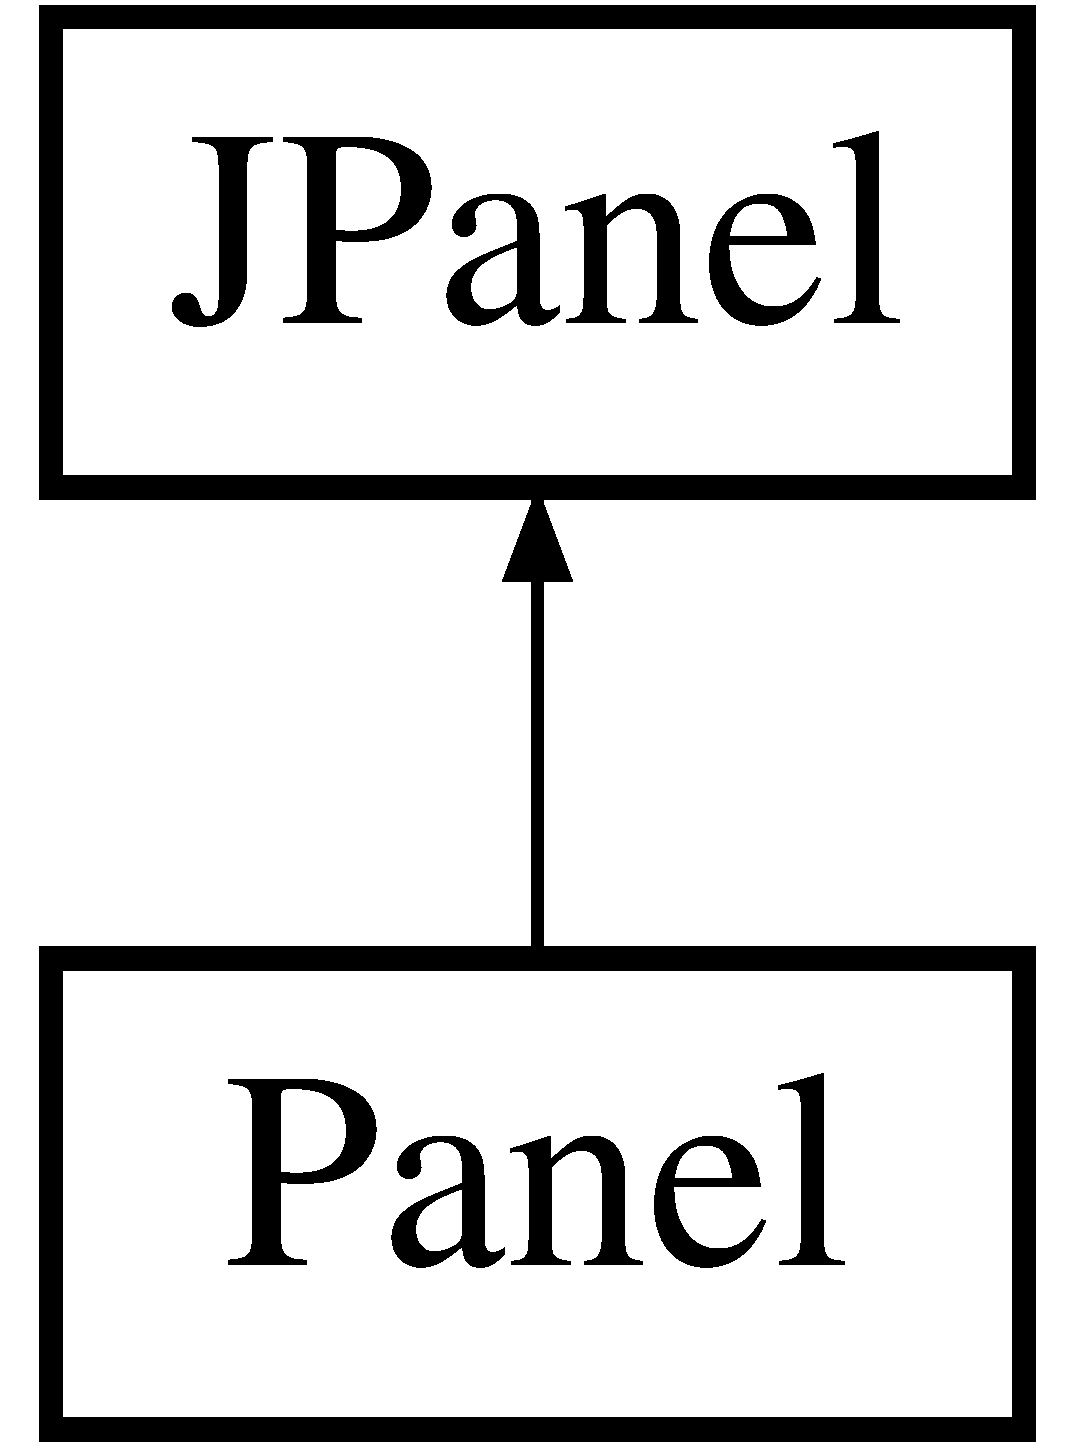
\includegraphics[height=2.000000cm]{class_panel}
\end{center}
\end{figure}
\subsection*{Public Attributes}
\begin{DoxyCompactItemize}
\item 
\hypertarget{class_panel_a893b671ec8c1dfd47189ab76b01e20c4}{}J\+Button {\bfseries load\+Button} = new J\+Button(load\+File)\label{class_panel_a893b671ec8c1dfd47189ab76b01e20c4}

\item 
\hypertarget{class_panel_a7157fd97c34255fa5e7498339a596d20}{}J\+Button {\bfseries go\+Button} = new J\+Button(go)\label{class_panel_a7157fd97c34255fa5e7498339a596d20}

\item 
\hypertarget{class_panel_aabf11270242e441dcc93b95590d92844}{}J\+Button {\bfseries delete\+Button} = new J\+Button(delete)\label{class_panel_aabf11270242e441dcc93b95590d92844}

\end{DoxyCompactItemize}


\subsection{Detailed Description}
Clase que recoge el contenido que mostrar� la ventana y las funcionalidades de este \begin{DoxyAuthor}{Author}
Bianney 
\end{DoxyAuthor}


The documentation for this class was generated from the following file\+:\begin{DoxyCompactItemize}
\item 
src/main/java/Panel.\+java\end{DoxyCompactItemize}

\hypertarget{class_tokenizer_main}{}\section{Tokenizer\+Main Class Reference}
\label{class_tokenizer_main}\index{Tokenizer\+Main@{Tokenizer\+Main}}
\subsection*{Static Public Member Functions}
\begin{DoxyCompactItemize}
\item 
static void \hyperlink{class_tokenizer_main_ad2ea4896c797112ff692834ab67fc186}{tokenizer} (File input, File output)
\end{DoxyCompactItemize}


\subsection{Detailed Description}
Clase que contiene el c�digo \char`\"{}tokenizador\char`\"{} \begin{DoxyAuthor}{Author}
Bianney 
\end{DoxyAuthor}


\subsection{Member Function Documentation}
\hypertarget{class_tokenizer_main_ad2ea4896c797112ff692834ab67fc186}{}\index{Tokenizer\+Main@{Tokenizer\+Main}!tokenizer@{tokenizer}}
\index{tokenizer@{tokenizer}!Tokenizer\+Main@{Tokenizer\+Main}}
\subsubsection[{tokenizer(\+File input, File output)}]{\setlength{\rightskip}{0pt plus 5cm}static void Tokenizer\+Main.\+tokenizer (
\begin{DoxyParamCaption}
\item[{File}]{input, }
\item[{File}]{output}
\end{DoxyParamCaption}
)\hspace{0.3cm}{\ttfamily [static]}}\label{class_tokenizer_main_ad2ea4896c797112ff692834ab67fc186}
Funci�n que ejecuta el tokenizador 
\begin{DoxyParams}{Parameters}
{\em input} & Archivo de entrada con la uni�n del texto de los distintos ficheros de entrada. \\
\hline
{\em output} & Archivo de salida, contendr� el texto separado en tokens. \\
\hline
\end{DoxyParams}


The documentation for this class was generated from the following file\+:\begin{DoxyCompactItemize}
\item 
src/main/java/Tokenizer\+Main.\+java\end{DoxyCompactItemize}

%--- End generated contents ---

% Index
\backmatter
\newpage
\phantomsection
\clearemptydoublepage
\addcontentsline{toc}{chapter}{Index}
\printindex

\end{document}
